Le modèle de notre application sera constitué d'une base de donnée \sql. Nous avons défini son architecture dans le diagramme \ref{fig::schema_bdd} tel que suit:

\begin{figure}[h!]
	\centering
	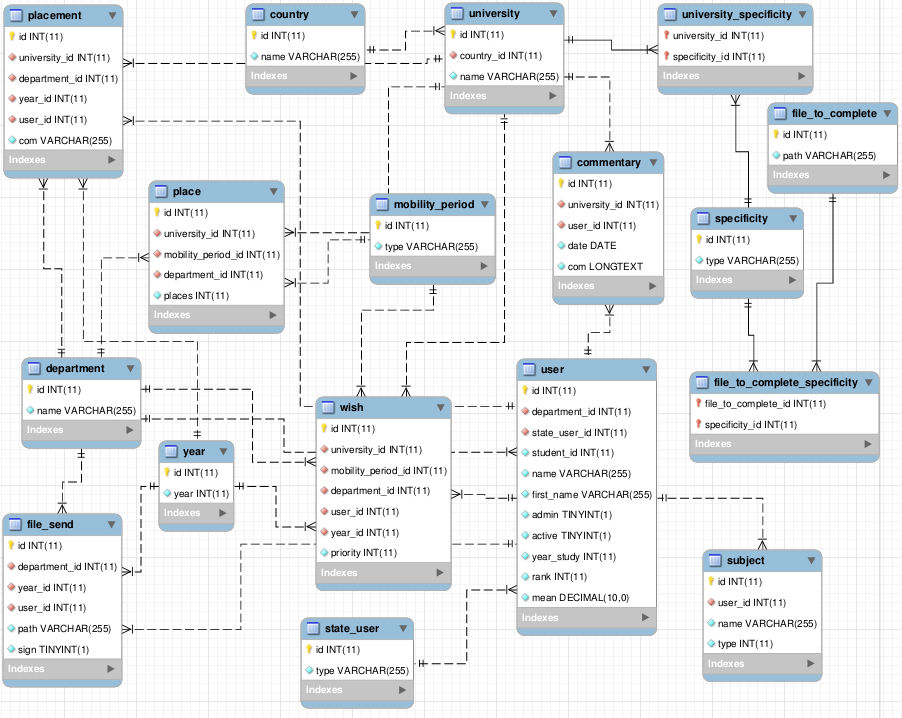
\includegraphics[scale=0.5]{ArchitectureLogicielle/SchemaBDD.png}
	\caption{Diagramme de l'architecture logicielle de l'application}
	\label{fig::schema_bdd}
\end{figure}


\section{Les modules}
Plusieurs informations importantes sont présentes dans cette base. Chacune de ces nœuds formera un bundle : 
\begin{itemize}
\item les utilisateurs ;
\item les universités ;
\item les fichiers ;
\item les affectations.
\end{itemize}
Un dernier bundle contiendra les vues principales et diverses.

\subsection{Utilisateur}

Nous utiliserons le bundle FOSUser qui contient des méthodes et une structure de donnée développée pour gérer les utilisateurs.
Les utilisateurs possèdent un état qui défini leur avancement dans la procédure d'affectation. C'est lui qui déterminera la vue d'accueil qui s'affichera pour l'étudiant. 
Chaque année, après une action d'un administrateur, les étudiants seront chargés depuis le LDAP pour mettre à jour la base de données et définir si un étudiant a redoublé ou non.
Ces utilisateurs sont assurés d'être uniques pour toujours grâce à leur id étudiant.

\subsection{Universités}

Les universités possèdent des spécificités qui serviront pour les tris dans les vues (TOEFL, Europe, etc).
Elle sont associées à une classe Place qui permet de définir le nombre de places disponibles pour un département à un semestre donné (ou double diplôme). Une université pouvant proposer plusieurs types de mobilité, cette classe est séparée.
Il existera dans le futur une classe pour définir les informations sur la page de chaque université, mais ne sachant pas encore exactement les champs nécessaire, nous n'avons pas encore implémenté la classe.

\subsection{Fichiers}

Il y a deux types de fichiers à gérer, les fichiers vierges mis à disposition des élèves et ceux qui sont complétés.

Certains fichiers vierges peuvent être associé à des spécificités (Learning Agreement pour les destinations Erasmus par exemple). Ils seront donc proposés par défaut lors de l'affectation à une université.
Les fichier à compléter sont liés à l'année et au département pour permettre de les garder en base un certain temps et les trier relativement facilement.

\subsection{Affectation}

Dans cette partie nous trouvons les \voe et le placement d'un candidat. Les \voe sont lié au département et à l'année en plus de l'utilisateur pour permettre là aussi un historique.
Le placement est l'endroit définitif où l'étudiant est affecté. Il possède aussi la problématique de l'historique.

\subsection{Vues principales}

Il reste l'année et les département. 
Il existera un département \textbf{ALL} pour permettre de définir un nombre de places disponibles commun à toute l'INSA, et non pas à un seul département.

\section{Architecture de l'application}

Le diagramme \ref{fig::archi_logicielle} présente les différents éléments qui composent notre application. Nous avons donc le serveur web, \textit{Nginx}, qui fait le lien entre la base de donnée \mdb et l'application développée en \symfony. Ceux-ci communiquent à l'aide du driver pdo de la base de donnée. De plus, le bundle Doctrine s'occupe des requêtes \sql de façon transparente.

De l'autre côté nous avons représenté le navigateur web de l'utilisateur. Il pourra afficher les vues envoyées par le protocole HTTP et générées à l'aide du bundle Twig.

\begin{figure}[h!]
	\centering
	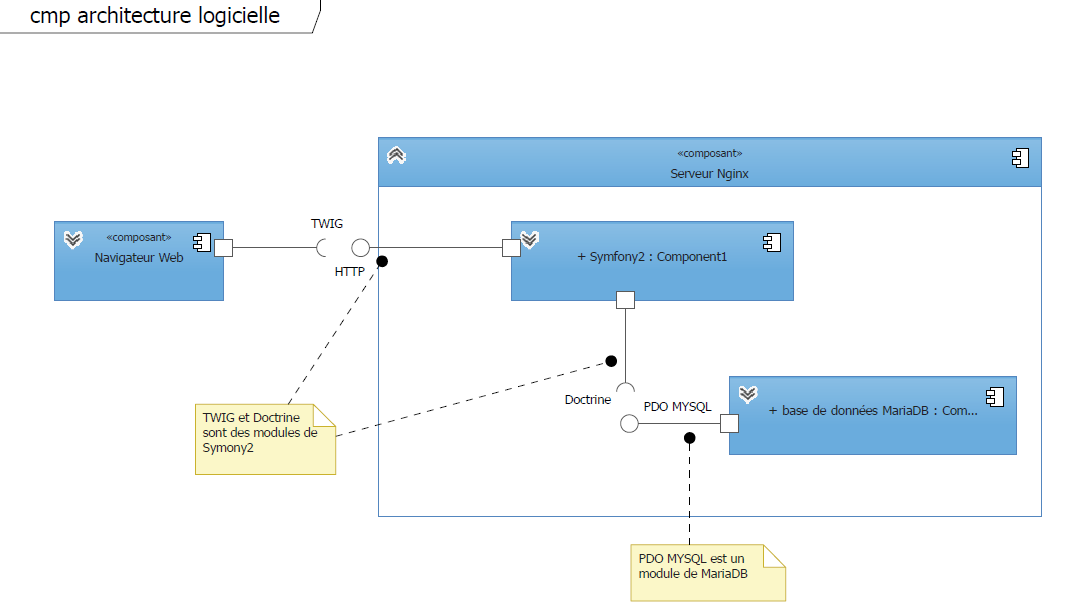
\includegraphics[scale=0.5]{ArchitectureLogicielle/archi_logicielle.png}
	\caption{Diagramme de l'architecture logicielle de l'application}
	\label{fig::archi_logicielle}
\end{figure}